\chapter{Implementation}

%\subsection{Coarse-graining engine}
The package consists of two parts: a C++ kernel and a scripting engine. The kernel is capable of processing atomistic topologies and trajectories and offers a flexible framework for reading, manipulating and analyzing of MD/SD/MC topologies and trajectories. It is modular: new file formats can be integrated without changing the existing code. Currently, an interface for \gromacs~\cite{gromacs4} topologies and trajectories is provided. 
%
The kernel also includes various coarse-graining tools, for example calculations of probability distributions of bonded and non-bonded interactions, correlation and autocorrelation functions, and updates for the coarse-grained pair potential. 
 
The scripting enginge is used to steer the iterative procedures. Here the analysis tools of the package used for sampling (e.g. \gromacs) can be integrated into the coarse-graining workflow, if needed.

The coarse-graining workflow itself is controlled by several Extensible Markup Language (\xml) input files, which contain mapping and other options required for the workflow control. In what follows, these input files are described.


\section{Mapping}
\label{sec:mapping}
{\em Mapping definitions} describe how to map a single molecule from an atomistic to a coarse-grained representation. A mapping definition has to be specified only once per molecule. The file contains sections for coarse-grained beads, bonded interactions in the coarse grained scheme as well as mapping matrices. If a system contains several molecule types, it has to be enssured that molecule names are set properly. The mapping files should be specified in a list separated by ; (e.g. "protein.xml;solvent.xml"). The \mapopt{ident} tag in the mapping definition must match the name of the molecule in the reference system.

The mapping file has similar entries as a topology, but contains additional information for mapping are present. In the topology section, coarse grained beads and bonded interactions are defined. Each coarse grained bead has a name, type and mapping entry, as well as a list of atoms which are mapped to it. The name must be unique within the mapping file. Type defines the type of the bead. The \mapopt{mapping} tag defines which mapping scheme is used from the mapping section in the file. Type and mapping can be different since the number of atoms for the same bead type may differ, e.g. at chain ends for saturating hydrogen atoms.

In the \mapopt{mapping} section, the mapping operator is defined. Currently this includes only weights for a linear mapping scheme.

A complete reference for mapping file definitions can be found in ref.~\ref{sec:ref_mapping}. To map from an atomistic to a reference system, \textbf{csg\_map} can be used:
\begin{verbatim}
  csg_map --top topol.tpr --trj traj.trr --cg "protein.xml;solvent.xml" --out cg.gro
\end{verbatim}

To create a coarse-grained topology based on the mapping scheme, see \textbf{csg\_gmxtopol}.

\subsection{Example - mapping file for propane}
\begin{figure}[ht]
  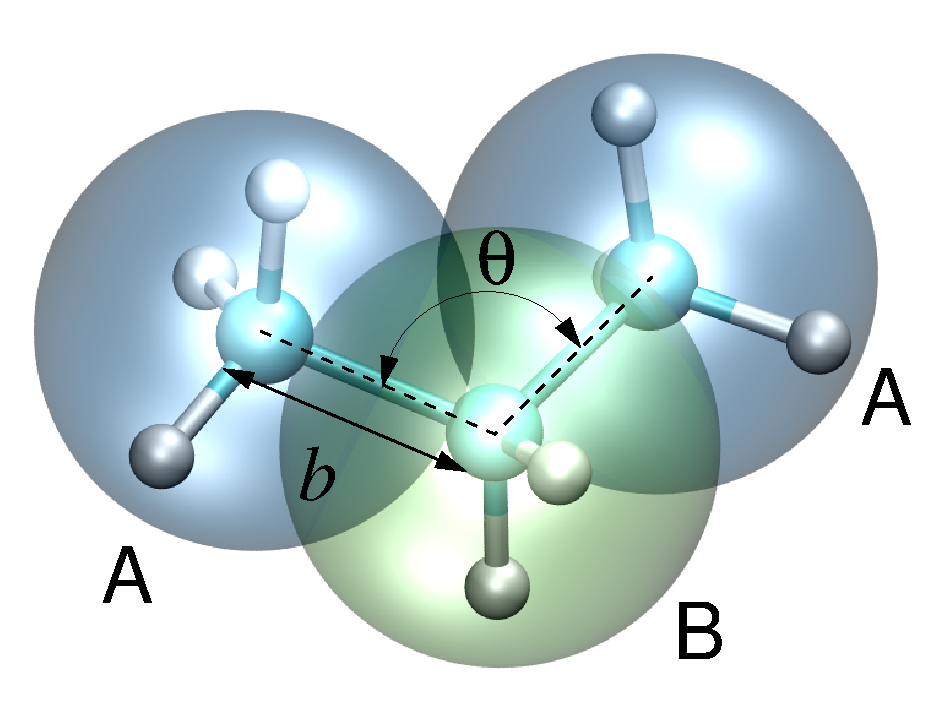
\includegraphics[width=0.4\textwidth]{functionality/fig/propane.eps}
  \caption{Mapping for propane}
\end{figure}

\lstinputlisting{functionality/propane.xml}


\section{Topologies}
A topology is defined as a set of beads with a certain bead type which are connected by bonded interactions.
\votca can read topologies in the \gromacs tpr format. However, it can also use a pdb file as topology, but, not all information are given or defined in this file format. If a pdb topology is used, it is recommended to fill in any additional molecule information using the xml advanced topology handling feature (see. \sect{sec:adv_topology})
\subsection{Manual topology handling}
\label{sec:adv_topology}
Many file formats do not have a clear definition of molecules. This can lead to problems, especially if a simulation contains several molecules with multiple types. Since during the coarse graining, the molecule type is identified by a name tag, names must also be set properly. \votca also offers the possibility to read a topology and later on modify parts of it. Everything is based on a definiton in an \xml topology file. This new \xml topology can then be used as topology in the \progopt{--tpr} option, as any other topology file. 

As \gromacs did not store molecule names in previous versions, but has introduced this feature in a newer release,  a recent .tpr file which contains molecule names should always be provided. For old topologies, rerun \gromacs \textbf{grompp} if possible to get a recent file. 

If no molecule information is present at all, it has to be manually defined. An example for a topology file that reads in last.pdb and then creates proper molecule definitions is:
\begin{lstlisting}
<topology base="last.pdb">
  <molecules>
    <clear/>
    <define name="mCP" first="1" nbeads="52" nmols="216"/>
  </molecules>
</topology>
\end{lstlisting}
where $<$clear/$>$ clears all molecule information that were present before.

If molecule information is already present in the parent topology, but molecule do not have proper names, molecules can be renamed. A short example is
\begin{lstlisting}
 <topology base="topol.tpr">
   <molecules>
     <rename name="PPY3" range="1:125"/>
     <rename name="Cl" range="126:250"/>
   </molecules>
 </topology>
\end{lstlisting}
Here, first the file topol.tpr is loaded, subsequently, molecules are renamed.

\subsection{Trajectories}
A trajectory is defined as a set of frames containing coordinates and eventually velecities and forces for the beads of a topology.
\votca currently supports trr, xtc, pdb and gro as trajector formats.

\section{Iterative workflow control}

\begin{figure}
  \includegraphics[width=0.7\columnwidth]{functionality/fig/flowchart.eps}
  \caption{
    \label{fig:flowchart}
    Block-scheme of the workflow control for the iterative methods. The most time-consuming parts are marked in red.
  }
\end{figure}

During the global initialization the initial guess for the coarse-grained potential is calculated from the reference radial distribution function or converted from a given potential guess to the internal format. The actual iterative step starts with an iteration initialization. It searches for possible checkpoints and copies and converts files from the previous step and the base directory. Then the simulation run is prepared by converting potentials to the format required by the external sampling program and the actual sampling is performed. Currently, an interface with \gromacs~\cite{gromacs4} is implemented but an extension for other packages is straightforward. After sampling the phasespace, the potential update $\Delta U$ is calculated. Often the update requires postprocessing, such as smoothing, interpolation, extrapolation or fitting to an analytical form. A simple pressure correction~\cite{Reith:2003} can also be seen as a postprocessing of $\Delta U$, due to the fact that it only adds a linear interparticle separation function.
%
Finally, the new potential is determined and postprocessed. If the iterative process continues, the next iterative step starts to initialize.

\subsection{General usage}
To setup the environment, run:
csh, tcsh:
\begin{verbatim}
  source <csg-installation>/bin/CSGRC.csh
\end{verbatim}
\begin{verbatim}
  bash: source <csg-installation>/bin/CSGRC.bash
\end{verbatim}
The program to run all iterative procedures is \prog{csg_inverse}. Tutorials can be found on the \votca homepage \votcaweb. 

\subsection{Run preparation}
To run the iterations, the input for the sampling program (e.g. \gromacs ) has to be prepared in order to carry out one iteration. All files for running a coarse-grained simulation except for the tabulated potentials that will be created during the run must be present and specified in the options xml-file.

As a target distribution, any table file can be given (e.g. gromacs output from g\_rdf). The program automaticaly takes care to resample the table to the correct grid spacing as specified in the .xml file.
The initial guess is created by inverting the tiven rdf. It is located in step\_000/$<$name$>$.pot.new. To specify the initial guess for a specific interaction by hand, write the potential table to a file called $<$name$>$.pot.in in the folder where you plan to run the iterative procedure.

To define which interactions are iteratively refined, a section for each has to be specified in the options file. A full list of parameters can be found in ref.~\ref{sec:ref_options}.

\subsection{Running the iterative process}
After all input files have been set up, the run can be started with
\begin{verbatim}
  csg_inverse <settings.xml>
\end{verbatim}

For each iteration, a separate directory (\textit{step\_$<$iteration$>$}) is created, where \textit{step\_000} has the special meaning of the initial setup before the first iterations. For each new iterations, the files required to run the CG simulation (as specified in the config file) are copied to the current working directory. Also the updated potentials from the last steps (step\_$<$n-1$>$/$<$interaction$>$.pot.new) are copied and used as the new working potentials (stetp\_$<$n$>$\/$<$interaction$>$.pot.cur).

After the preparation, all potentials are converted to the format of the sampling program and the simulation is started. As soon as the run is finished, analysis programs are started and new distributions ($<$interaction$>$.dist.new) as well as the update ($<$interaction$>$.dpot.new) are calculated. Before \votca adds the update to the old potential, the update can be processed in the post\_update step. For each script that is specified in post\_update, \votca renames $<$interaction$>$.dpot.new to $<$interaction$>$.dpot.old, stores it in $<$interaction$>$.dpot.$<$a-number$>$, and calls the processing script. Each processing script is supposed to take the current update ($<$interaction$>$.dpot.cur) and write the processed update ($<$interaction$>$.dpot.new). Pressure correction is implemented as a post\_update script within this framework.

After all post\_update scripts have been called, the update is added to the potential and the new potential ( $<$interaction$>$.pot.new ) is written. Furthermore, processing of the potential is performed in the post\_add step, analogous to the tasks performed in post\_update but now for the potential instead of the update.

In summary, the standard output files of \votca for each step are listed in the following table:

\begin{tabular}{ll}
*.dist.new & distribution functions of the current step \\
*.dpot.new & the final potential update, created by calc\_update \\
*.dpot.$<$number$>$ & for each post\_update script, the current .dpot.new is saved and a new one is created\\
*.pot.cur & the current potential, which the actual run was performed with \\
*.pot.new & the new potential after the add step \\
*.pot.$<$number$>$ & same as dpot.$<$number$>$ but for post\_add
\end{tabular}

If some sub-step within one iteration has failed, additional information can be found in the log file. The name of this log file can be specified in the options xml-file.

\subsection{Run continuation}
There are two scenarios when one wants to continue a run. Either, that of extending a finished run or that the run was interrupted and one needs to restart at the current point. When \prog{csg_inverse} is started, it automatically checks for a file called \textit{done} in the current directory. If it exists, the program assumes that the run is finished. To extend the run, simply increase \cgopt{inverse.iterations_max} in the settings file and remove the file called done. After that, csg\_inverse can be restarted, it will automatically recognize existing steps and continue after the last one.

If a run was interrupted, \prog{csg_inverse} might not be able to restart on its own. In this case, the easiest solution is just to delete the last step and start again. It will then redo the last step and continue. However, this method is not always practical since sampling and analysis might take a very long time and the run might have only crashed due to some bogus post processing option. To avoid redoing the entire run, \prog{csg_inverse} creates a file with restart points, which marks actions in the step that were already completed (like simulation, analysis, etc). The file is specified in the option \cgopt{inverse.restart_file}. If specific actions should be redone, lines in that file can also removed by hand. In addition, a file \textit{done} is created in each folder for a steps which have already been finished.

\subsection{Customization}
In principle, each sub-step of an iteration and all direct calls can be changed. 
All script is called via two keywords.
\begin{verbatim}
  csg_call key1 key2
\end{verbatim} 
For example \texttt{csg\_call update imc} calls the update script for inverse monte carlo procedure.
The default keyword to script mapping can be seen in \sect{sec:csg_table} or seen directly by calling:
\begin{verbatim}
  csg_call --list
\end{verbatim} 

Please {\em never} change the scripts in the \votca installation. It is better to copy the script to your script directory (defined by \cgopt{inverse.scriptdir}) and redirect its call by creating a own \texttt{csg\_table} in this directory with a contain like this:
\begin{verbatim}
  key1 key2 script options
  key3 key4 script2
\end{verbatim} 
One can even overload existing call.
\subsubsection{An useful example}
\prog{csg_inverse} runs \prog{mdrun} from the \gromacs package only on one cpu and we want to change that due to the fact that we have 8 cpu machine and want to save some time.
First we try to find out which script calls \prog{mdrun}:
\begin{verbatim}
  csg_call --list | grep gromacs
\end{verbatim}
In this case we are lucky, the output is quite helpful:
\begin{verbatim}
  init gromacs initalize_gromacs.sh
  prepare gromacs prepare_gromacs.sh
  run gromacs run_gromacs.sh
  pressure gromacs calc_pressure_gromacs.sh
  rdf gromacs calc_rdf_gromacs.sh
  imc_stat gromacs imc_stat_generic.sh
  convert_potential gromacs potential_to_gromacs.sh
  functions gromacs functions_gromacs.sh
\end{verbatim}
the third entry sounds reasonable. If the output of \prog{csg_call} is not useful, one should try to find the right script in \sect{sec:csg_table}. If this doesn't help one has to go the $<$csg-installation$>$/share/scripts/inverse and find the script there. However in this case the output of:
\begin{verbatim}
  csg_call --show run gromacs
\end{verbatim}
looks like we have found the right script:
\begin{verbatim}
  #!/bin/bash
  # Copyright 2009 The VOTCA Development Team (http://www.votca.org)
  #
  # Licensed under the Apache License, Version 2.0 (the "License");
  # you may not use this file except in compliance with the License.
  # You may obtain a copy of the License at
  #
  #     http://www.apache.org/licenses/LICENSE-2.0
  #
  # Unless required by applicable law or agreed to in writing, software
  # distributed under the License is distributed on an "AS IS" BASIS,
  # WITHOUT WARRANTIES OR CONDITIONS OF ANY KIND, either express or implied.
  # See the License for the specific language governing permissions and
  # limitations under the License.
  #

  if [ "$1" = "--help" ]; then
  cat <<EOF
  ${0##*/}, version 1.0_rc1 hgid: 5553f40f6aafbc05449582c788fd5017c72c9b7b
  This script runs gromacs
  for the Inverse Boltzmann Method

  Usage: ${0##*/}

  USES: run_or_exit mdrun
  EOF
     exit 0
  fi

  check_deps "$0"

  run_or_exit mdrun
\end{verbatim}
Now we create our own scriptdir, add script there, make it executable and overload the call of the script:
\begin{verbatim}
  mkdir -p SCRIPTDIR
  csg_call --show run gromacs > SCRIPTDIR/MY_run_gromacs.sh
  chmod 755 SCRIPTDIR/MY_run_gromacs.sh
  echo "run gromacs MY_run_gromacs.sh" >> SCRIPTDIR/csg_table
\end{verbatim}
Please note that \texttt{MY\_run\_gromacs.sh} is the name of the script and \texttt{SCRIPTDIR} is the custom script directory, which can be a global or local path.
Now we change the last line of \texttt{MY\_run\_gromacs.sh} to:
\begin{verbatim}
  run_or_exit mpirun -np 8 mdrun
\end{verbatim}
and that is it, please note that you should be remove the license infomations and change the version of the scipt to not end up in a big mess.
You can check your work by running:
\begin{verbatim}
  csg_call --scriptdir SCRIPTDIR --list
  csg_call --scriptdir SCRIPTDIR --show run gromacs
\end{verbatim}
and do not forget to add \texttt{SCRIPTDIR} to \cgopt{inverse.scriptdir} in setting \xml file (see \sect{sec:ref_options}).






